\documentclass[12pt]{article}

\usepackage[english]{babel}
\usepackage[utf8]{inputenc}
\usepackage{fancyhdr}

\usepackage[margin=1.5in]{geometry}
\usepackage{pgf}
\usepackage{pgfplots}
\usepackage{siunitx}
\usepackage{tikz}
\usepackage{float}
\usepackage{amsmath}

\usepackage[font=small,labelfont=bf]{caption}
\usepackage{pstricks-add}
\usepackage{pgfplotstable}
\usepackage{filecontents}
\usepackage{pgfplotstable}

\usetikzlibrary{scopes}
\usetikzlibrary{angles,quotes}
\usetikzlibrary{calc}
\pgfplotsset{compat=1.5}

\newcommand*{\I}{\imath}
\newcommand*{\J}{\jmath}
\newcommand{\norm}[1]{\lvert #1 \rvert}

\begin{filecontents}{data1.csv}
    X	   F
    1	113.778
    2	12.698
    3	3.679
    4	1.539
    5	0.784
    6	0.453
    7	0.285
    8	0.19
    9	0.134
    10	0.097
    11	0.073
    12	0.056
    };
\end{filecontents}

\begin{document}
\sisetup{per-mode=symbol}

\begin{titlepage}
    \begin{center}
        \vspace*{1cm}
        \textbf{Electric Dipoles}

        \vspace{0.5cm}
        Lab: 01

        \vspace{1cm}

        \textbf{Jaden Moore}

        \vfill

        Orange Coast College\\
        Physics A280L\\
        February 15th, 2021

    \end{center}
\end{titlepage}

\pagestyle{fancy}
\fancyhf{}
\setlength{\headheight}{15pt}
\lhead{Electric Dipoles}
\rhead{Lab: 01}
\cfoot{\thepage}

\section{Introduction}
In this lab, we analyze the force exerted by an electric dipole onto a point charge as the distance between the two increases. We then compare the experimental force with the theoretical force exerted by the dipole and calculate the percent error between them.

\section{Electric Dipoles}
Consider two equal and opposite point charges $\pm \vec{q}$ positioned very close together, separated by a small distance $2a$ such that it forms an electric dipole. We then position a point charge $\vec{Q}$ some large distance $x$ away such that $x>>a$:

\setlength{\tabcolsep}{1pt}
\renewcommand{\arraystretch}{1}
\newcolumntype{P}[1]{>{\centering\arraybackslash}p{#1}}

\begin{figure}[H]
    \centering

    \caption[10pt]{A system of an electric dipole and a point charge $Q$ where $x>>a$}

    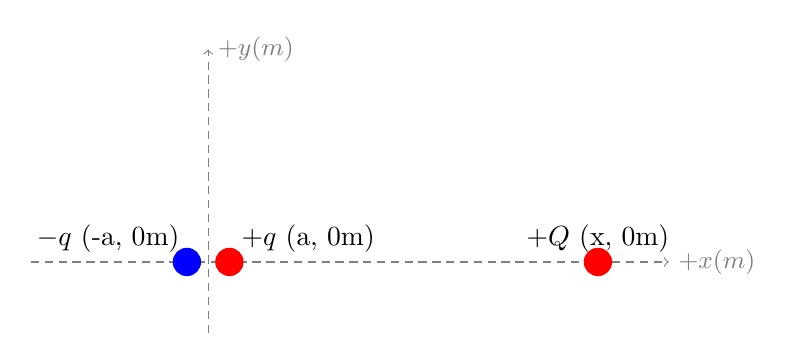
\begin{tikzpicture}[scale=0.9]
        \begin{scope}

            {[densely dashed,gray,font=\small,->]
                \draw (-5, 0) -- (4,0) node[right] {$+x (m)$};
                \draw (-2.5,-1) -- (-2.5,3) node[right] {$+y (m)$};
            }

            \fill[blue] (-2.8,0) circle (2mm) node[above, shift={(-1,0)}, black]{$-q$ (-a, 0m)};
            \fill[red] (-2.2,0) circle (2mm) node[above, shift={(1,0)}, black]{$+q$ (a, 0m)};

            \fill[red] (3,0) circle (2mm) node[above, black]{$+Q$ (x, 0m)};

        \end{scope}
    \end{tikzpicture}
\end{figure}

If we let $k = \SI{9e+9}{\newton\metre\squared\per\coulomb\squared}$, Coulomb's constant and $\vec{p} = q(2a)\hat{\I}$, the electric dipole moment, we find that the theoretical force exerted by the electric dipole onto the point charge $Q$ is:
\begin{equation} \label{eq1}
    \vec{F} = \frac{2k p Q}{x^3} \hat{\I}
\end{equation}


\subsection{Data}
Below we put into a table the data collected by measuring the force exerted onto the point charge $Q$ by the electric dipole at different distances. In order to collect this data, we use the Physlet\textregistered \space Physics dipole simulation 22.3 and measure the distance with a mouse.

\setlength{\tabcolsep}{2pt}
\renewcommand{\arraystretch}{1.2}

\begin{figure}[H]
    \begin{center}
        \begin{tabular}{ P{5cm} P{5cm} }
            \hline
            \multicolumn{2}{c}{Table 1: Force exerted onto Q as x increases} \\
            \hline  
            Distance $[x(m)]$ & Force $[F(N)]$                              \\
            \hline
            1              & 113.778                                        \\
            2              & 12.698                                         \\
            3              & 3.679                                          \\
            4              & 1.539                                          \\
            5              & 0.784                                          \\
            6              & 0.453                                          \\
            7              & 0.285                                          \\
            8              & 0.190                                          \\
            9              & 0.134                                          \\
            10             & 0.097                                          \\
            11             & 0.073                                          \\
            12             & 0.056                                          \\
            \hline
        \end{tabular}
    \end{center}
\end{figure}

\subsection{Data Analysis}
A preliminary analysis of the data indicates that as the distance between the electric dipole and the point charge increases, the force exerted onto the point charge decreases exponentially. This data is conclusive with the formula of the theoretical force which shows that the force falls of proportionally with the inverse cube of the distance $x$ as seen in Equation 1.

\subsection{Graph}
Now consider the data gathered in Table 1 in the form of a power regression line graphed below.

\begin{figure}[H]
    \centering

    \caption[10pt]{Force exerted on a point charge over distance}

    \begin{tikzpicture}
        \pgfplotsset{width=10cm,
            legend style={font=\footnotesize}}
        \begin{axis}[
                xlabel={Distance $[x(m)]$},
                xmin=0,
                xmax=12,    
                ylabel={Force $[F(N)]$},
                ymin=0,
                ymax=120,
                yticklabel=\pgfmathprintnumber{\tick},
                legend cell align = left,
                legend pos = north east,
            ]
            \addplot[only marks] table[x=X,y=F]{data1.csv};
            \addplot[black,smooth,domain=0.98:12] {108.13*x^-3.051};
            \addlegendimage{only marks}
            \addlegendentry{force over distance}
            \addlegendimage{no markers, red}
            \addlegendentry{power regression fit}
        \end{axis}
    \end{tikzpicture}
\end{figure}

\paragraph{}

From the power regression we get the general equation of the line of best fit to be:

\[F=\frac{108.13}{x^{3.051}}\]

\subsection{Graph Analysis}
An analysis of Figure 2 indicates that when the point charge $Q$ is very close to the dipole, a very small change in $x$ yields very large changes in $F$. In theory, we said that the force exerted by the dipole falls of as $\frac{1}{x^3}$ of the distance. The power fit yielded a value of $\frac{1}{x^{3.051}}$ of the distance which is very close to the theoretical values. We are able to calculate the percent error between these values as such:
\[\%error = \frac{\norm{3.051-3.000}}{3.000} (100) = 1.7\%\]
This indicates that our power regression line produces a 1.7 percent error with respect to the theoretical value. Furthermore, we notice that the value $2kpQ$ = $\SI{108.13}{\newton\metre\cubed}$ from Equation 1. Additionally, since we know that $Q$ is positively charged, we can determine that the charge on the right side of the dipole is positive because it creates a force which repels the positive point charge $Q$ away, which indicates that the positive charge is closer to $Q$ as depicted in Figure 1.
\section{Conclusion}
It appears that as the distance between a point charge and an electric dipole increases, the force exerted onto the point charge by the dipole decreases. In the experiment, we were able to prove this by measuring the force exerted onto the point charge at different distances away. We were able to find an equation from the graph using a power regression fit of the data, which turned out to be \[F=\frac{108.13Nm^3}{x^{3.051}m^3}\]
In theory, this force falls off with the inverse cube of the distance between them as seen in Equation 1. The experiment proves this by providing a similar figure of $\frac{1}{x^{3.051}m^3}$ with a percent error of 1.7\%. The greatest obstacle in the lab is trying to get data that you are happy with from the experiment. There will always be percentage errors involved when measuring with physical instruments. The biggest takeaway from the experiment is that while the force between two point charges falls off proportionally to the inverse \textit{square} of the distance, in the case of an electric dipole, it is the inverse \textit{cube} of the distance which is an interesting distinction.
\end{document}
